\documentclass[a4paper,11pt,article]{article}

\usepackage[margin=1in]{geometry}
\usepackage[utf8]{inputenc}
\usepackage{fourier}
\usepackage{amsmath,amssymb}

\usepackage{color}
\definecolor{orange}{rgb}{0.75,0.5,0}
\definecolor{magenta}{rgb}{1,0,1}
\definecolor{cyan}{rgb}{0,1,1}
\definecolor{grey}{rgb}{0.25,0.25,0.25}
\newcommand{\outline}[1]{{\color{grey}{\scriptsize #1}}}
\newcommand{\revnote}[1]{{\color{red}\textit{\textbf{#1}}}}
\newcommand{\note}[1]{{\color{blue}\textit{\textbf{#1}}}}
\newcommand{\citenote}[1]{{\color{orange}{[\textit{\textbf{#1}}]}}}

\usepackage{xspace}
\newcommand{\zfive}{\ensuremath{Z_{500}}\xspace}

\usepackage{listings}
\usepackage{courier}
\lstset{basicstyle=\tiny\ttfamily,breaklines=true,language=Haskell}

\usepackage{fancyvrb}
\usepackage{url}

\usepackage{tikz}
\usetikzlibrary{arrows,positioning}

\usepackage{natbib}

\DeclareMathOperator{\diag}{diag}
\DeclareMathOperator*{\argmax}{arg \, max}

\usepackage{subfig}
\usepackage{float}
\newfloat{listing}{tbp}{lop}
\floatname{listing}{Listing}

\title{Standalone ECBILT Experiments}
\author{Ian~Ross}
\date{13 January 2015 -- ???}

\begin{document}

\maketitle

%======================================================================
\section{Introduction}

The idea here is to do some experiments with a standalone version of
the ECBILT 3-level atmosphere model to decide whether it's a suitable
candidate for coupling into GENIE.  The two main things to consider
here are the speed of the ECBILT model and how good its climatology
is.  To investigate these things, I've done a quick first comparison
with a HadAM3 simulation (BRIDGE simulation \texttt{tcszd}).

There are two versions of ECBILT that could be used for this
comparison.  The first is already coupled into the LOVECLIM EMIC, so
would require some work to decouple it and set it up for standalone
operation.  The second is the original standalone ECBILT
model\footnote{Downloaded from here
  \url{http://knmi.nl/~selten/pro_ecbilt.html}.}, which is what I'm
going to start with.  It has a couple of deficiencies compared to the
version included in LOVECLIM, but it's good enough for a quick first
look.  The main deficiency of the standalone ECBILT version is that
it's not possible to change GHG forcings.  This is because of the way
the LW radiation scheme works: it's an empirical fit to LW radiation
absorption from the GFDL GCM.  I'm not yet sure what GHG conditions
that fitting was done against, but I'm going to press on assuming that
it was pre-industrial, as for the UM simulation.  For applications in
GENIE, we obviously need to be able to change the GHG concentrations
so, if results from the first experiments with the standalone ECBILT
are promising, I'll probably just transplant the newer LW radiation
scheme from the LOVECLIM version of ECBILT (which treats GHGs
explicitly) into the standalone ECBILT.

The approach I'm going to take to model validation here is just to
convert boundary conditions from a suitable HadAM3 run to the form
required to drive ECBILT, do the same sort of atmosphere-only
simulation as done in the HadAM3 job and to compare the parts of the
climatology most important for long-term GENIE simulations between the
two models (also looking at model performance along the way).

As a first simple attempt, I'm going to leave all ECBILT input files
unchanged from their defaults except for SST and sea-ice forcing,
which are adapted from the HadAM3 simulation.  This approach means
that there's no need to convert land/sea masks, land cover types, the
lake mask used by ECBILT, and so on.  If we decide to go further, I'll
do simulations using a land/sea mask and other boundary conditions
based on the HadAM3 data (probably also updating the ECBILT LW
radiation scheme as mentioned above).


%======================================================================
\section{Code and test platform setup}

All the experiments reported here are performed on a machine running
Arch Linux (rolling release as of 18 January 2015), with a 3\,GHz
Intel Core i5-3330 CPU and 16\,Gb of main memory.  All test runs were
performed on a lightly loaded machine.  Very few code changes were
needed to get the standalone ECBILT code to build with the compiler
used (GFortran 4.9.2).


%======================================================================
\section{Control experiment \#1}

\begin{itemize}
  \item{Run name: \texttt{control-expt-1}.}
  \item{Original standalone ECBILT code, with only minimal changes for
    compilation.}
  \item{SST and sea-ice forcing converted from UM \texttt{tcszd}
    experiment.}
  \item{Simulation length: 100 years; spin-up: 70 years; analysis: 30
    years.}
\end{itemize}

%----------------------------------------------------------------------
\subsection{Boundary conditions}

Boundary conditions to run the standalone ECBILT model were derived
from the BRIDGE \texttt{tcszd} HadAM3 simulation.  This is a 100-year
pre-industrial atmosphere-only simulation with prescribed
climatological SSTs and sea ice.

In order to get an initial ECBILT simulation set up quickly, I decided
to convert only the SST and sea ice forcing from the HadAM3
simulation, keeping the original ECBILT land/sea mask, orography, lake
mask and land surface conditions (e.g. albedo), GHG concentrations and
so on.  Modifying these latter conditions to match HadAM3 will take
more work than the relatively simple SST and sea ice regridding.  I'll
go ahead and do that if the results from the first simulation are
encouraging enough.

\begin{figure}
  \begin{center}
    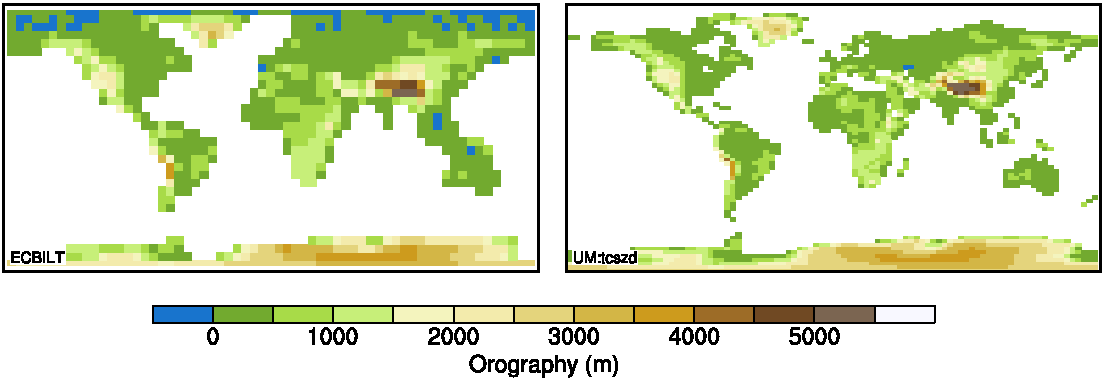
\includegraphics[width=\textwidth]{../control-expt-1/plots/orog-plots}
  \end{center}
  \caption{ECBILT and UM orography and land/sea masks used for
    comparison experiments.}
  \label{fig:orog}
\end{figure}

Figure~\ref{fig:orog} shows the land/sea mask and orography for ECBILT
and HadAM3 for comparison.  One comment needs to be made about the
ECBILT land/sea mask here: although some areas that should be ocean
are treated as land in the land/sea mask, in particular the
Mediterranean, the Great Lakes and the South China Sea, these grid
cells \emph{are} treated appropriately as water areas, via the use of
a seperate lake mask identifying grid cells that have a significant
water fraction.

\subsubsection{SST and sea-ice}

Conversion of SST and sea-ice from the HadAM3 boundary conditions to
the form needed by ECBILT is pretty straightforward.

For the SST, the HadAM3 boundary conditions are given as a monthly
climatology of SST.  ECBILT requires daily SST on a different grid, so
I take the HadAM3 monthly SST fields, Poisson fill to get rid of
missing values, regrid to the ECBILT grid, mask with the ECBILT
land/sea mask, then use independent periodic interpolation in time at
each grid point to generate a daily SST climatology.  This data is
then converted to the binary format read by ECBILT.

For sea ice, again HadAM3 again uses a monthly climatology, but ECBILT
uses a ``birth/death'' map showing, for each grid cell, the month of
the year where sea ice first appears and the month when it disappears.
To generate a sea ice driver file in this form, the HadAM3 monthly sea
ice data is first Poisson filled, regridded and masked to generate a
monthly sea ice climatology on the ECBILT grid.  Next, some simple
heuristics are used to determine ``birth'' and ``death'' months for
sea ice in each grid cell, and this information is encoded into the
ASCII file format used by ECBILT.

%% %----------------------------------------------------------------------
%% \subsubsection{Other boundary conditions}

%% \begin{itemize}
%%   \item{Conversion of boundary conditions (2): same plus land/sea
%%     mask, lake mask, orography, albedo, GHG concentrations, orbital
%%     parameters.}
%%   \item{Plots of land/sea mask compared between original ECBILT, UM
%%     and ECBILT-regridded UM mask.}
%% \end{itemize}


%----------------------------------------------------------------------
\subsection{Model performance}

The 100-year simulation performed here too about 75 minutes (wallclock
and CPU time were about the same), equating to \textbf{about 45
  seconds per year of simulation}.  Replacing the existing LW
radiation scheme in ECBILT with the more explicit scheme in the
LOVECLIM code will probably slow this down a little bit, but not much.

The ECBILT code is all serial, so there may be opportunities for
parallelisation if performance is a problem.  The atmosphere runs at a
longitude/latitude resolution of $64 \times 32$ using a spectral
method for stepping the dynamics.  I've not yet done any profiling to
determine where the best places to look for optimisations are, but
that would be the obvious thing to do.

%----------------------------------------------------------------------
\subsection{Model climatology}

Figures~\ref{fig:ts}--\ref{fig:wind} show seasonal climatologies of
surface temperature, precipitation, evaporation, $P-E$ and atmospheric
circulation for the ECBILT simulation alongside the same plots for the
HadAM3 \texttt{tcszd} simulation.

\paragraph{Surface temperature}

The large-scale patterns of surface temperature field in the ECBILT
simulation are pretty good.  Because of the SST forcing, it's a
relatively easy field to get right, but it does show that there are no
gross problems with the model.  What differences there are between the
ECBILT and HadAM3 fields appear mostly to be due to the rougher
orography in ECBILT -- the Tibetan plateau and western North America
near the Rockies are the areas where this is most obvious.

\begin{figure}
  \begin{center}
    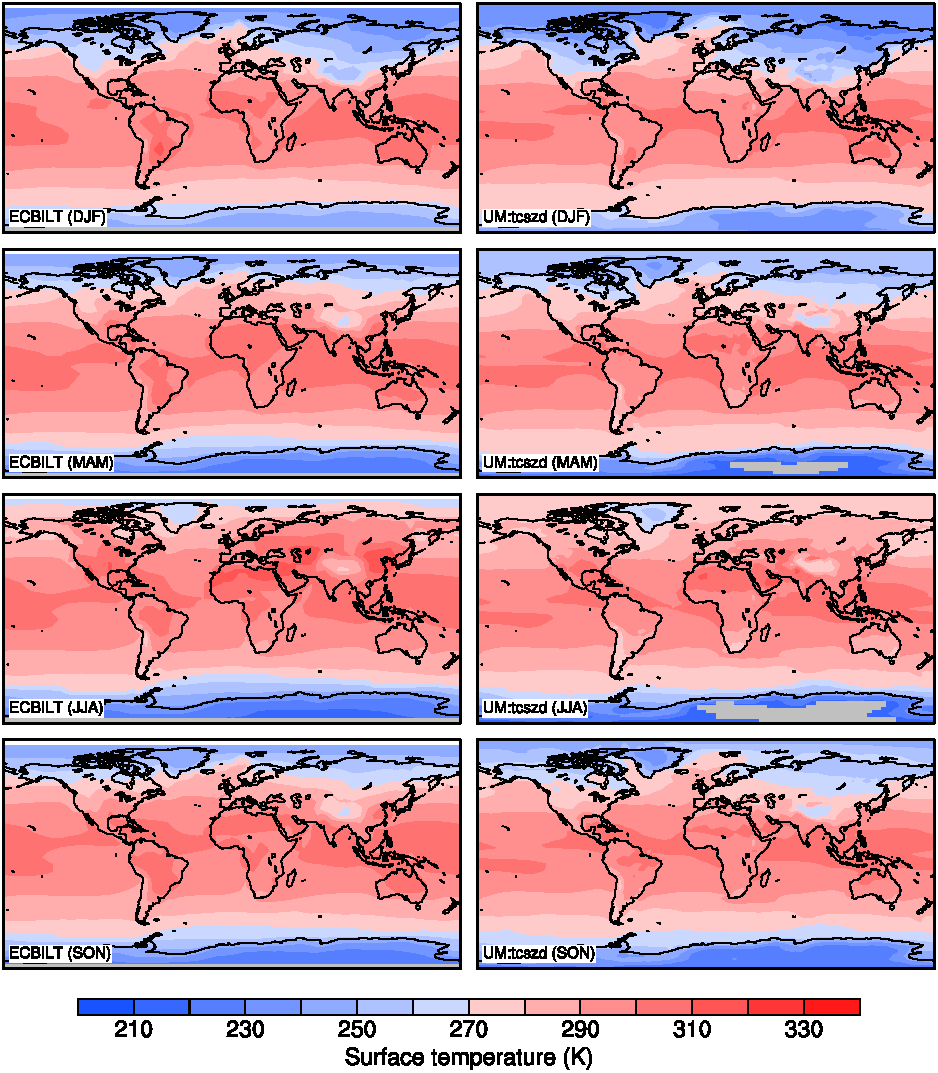
\includegraphics[width=\textwidth]{../control-expt-1/plots/ts-plots}
  \end{center}
  \caption{Seasonal surface temperature for ECBILT and UM comparison
    experiments.}
  \label{fig:ts}
\end{figure}

\paragraph{Precipitation}

The differences between the ECBILT and HadAM3 fields here are more or
less what you would expect from a comparison between a lower
resolution (in both the horizontal but also, more importantly, in the
vertical direction) and a higher resolution model.  Winter storm
tracks in the Atlantic are not well represented in ECBILT and tropical
convective precipitation is much less well localised in ECBILT, with a
large diffuse region of precipitation stretching from the western into
the central Pacific.  HadAM3 shows tropical precipitation much more
localised over the western Pacific warm pool and narrow bands either
side of the equator across the rest of the Pacific.  These kinds of
deficiencies in precipitation modelling are kind of inevitable in a
model with only three levels in the vertical.

\begin{figure}
  \begin{center}
    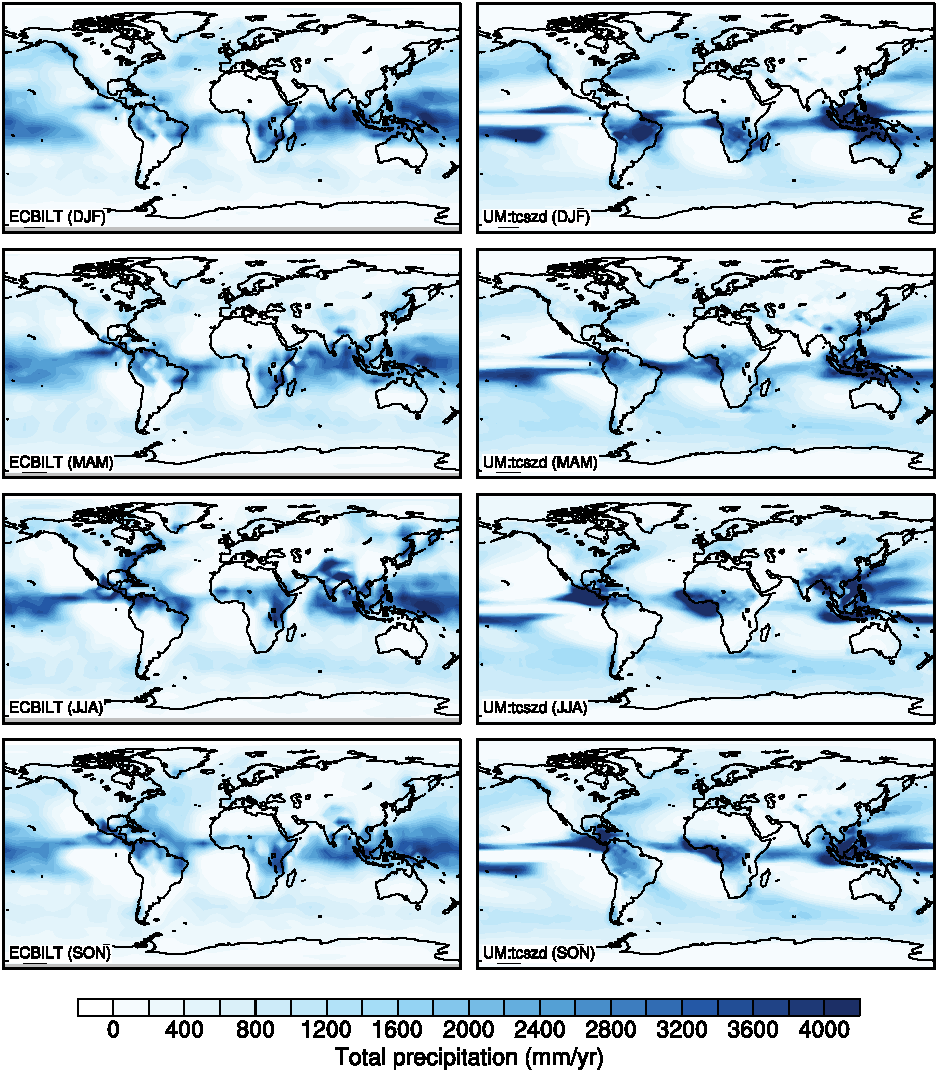
\includegraphics[width=\textwidth]{../control-expt-1/plots/pp-plots}
  \end{center}
  \caption{Seasonal precipitation for ECBILT and UM comparison
    experiments.}
  \label{fig:pp}
\end{figure}

\paragraph{Evaporation}

Similar comments apply here as to the precipitation comparison:
evaporation from the ocean is much less well spatially localised in
ECBILT, with a large region of the western Pacific showing high
evaporation values and no clear ITCZ being visible.  Again, hard to
get this right even in a model with more levels in the vertical, let
alone one with only three!

\begin{figure}
  \begin{center}
    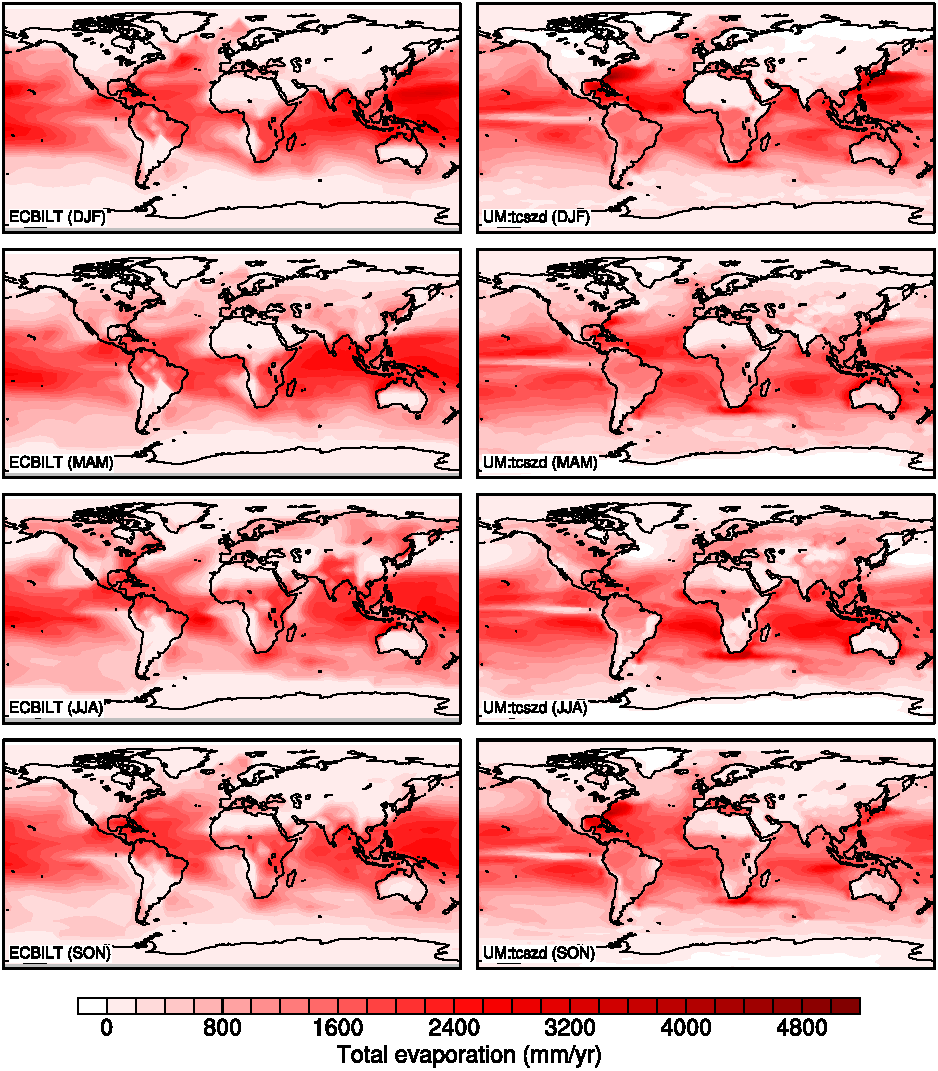
\includegraphics[width=\textwidth]{../control-expt-1/plots/evap-plots}
  \end{center}
  \caption{Seasonal evaporation for ECBILT and UM comparison
    experiments.}
  \label{fig:evap}
\end{figure}

\paragraph{$P-E$}

The spatial patterns of $P-E$ in ECBILT exhibit the same problems seen
in the individual precipitation and evaporation plots: the
hydrological cycle is generally much more spatially diffuse than in
the HadAM3 simulation (and in reality).  For both models, the mean
annual hydrological cycle is more or less balanced (for HadAM3 the
area-averaged annual imbalance is about $-2$\,mm and for ECBILT it's
about 23\,mm).  The patterns of $P-E$ in ECBILT are weaker and more
diffuse than HadAM3, although if you squint a little, the spatial
patterns of positive and negative moisture budget are more or less
right.

\begin{figure}
  \begin{center}
    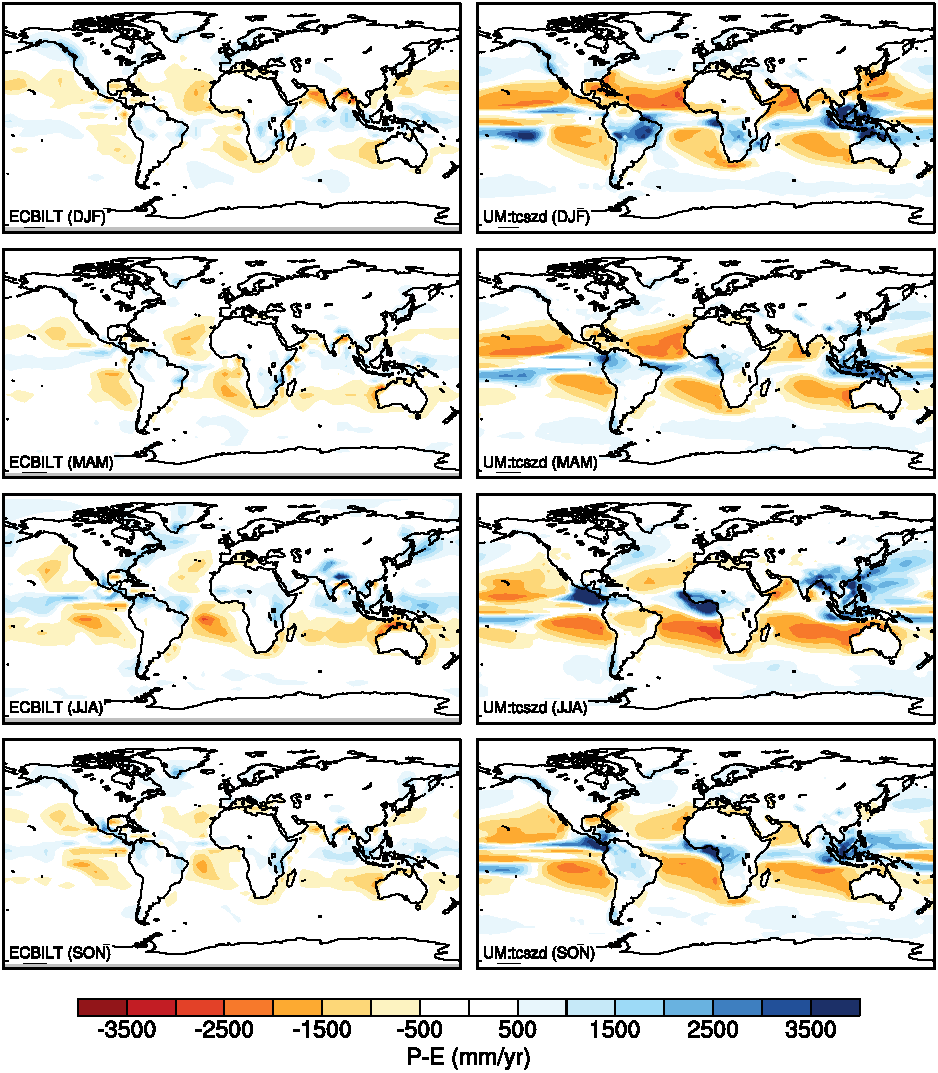
\includegraphics[width=\textwidth]{../control-expt-1/plots/pmine-plots}
  \end{center}
  \caption{Seasonal precipitation minus evaporation for ECBILT and UM
    comparison experiments.}
  \label{fig:pmine}
\end{figure}

\paragraph{Winds}

Finally, the distribution of upper and lower level winds and vertical
pressure velocity follow more or less the pattern that you would
expect: the atmospheric circulation in ECBILT is weaker and more
diffuse than in HadAM3, particularly in the vertical direction.  This
vertical smoothing because of the small number of vertical levels in
ECBILT is almost certainly the source of the weaker hydrological cycle
seen in the $P-E$ plots.

\begin{figure}
  \begin{center}
    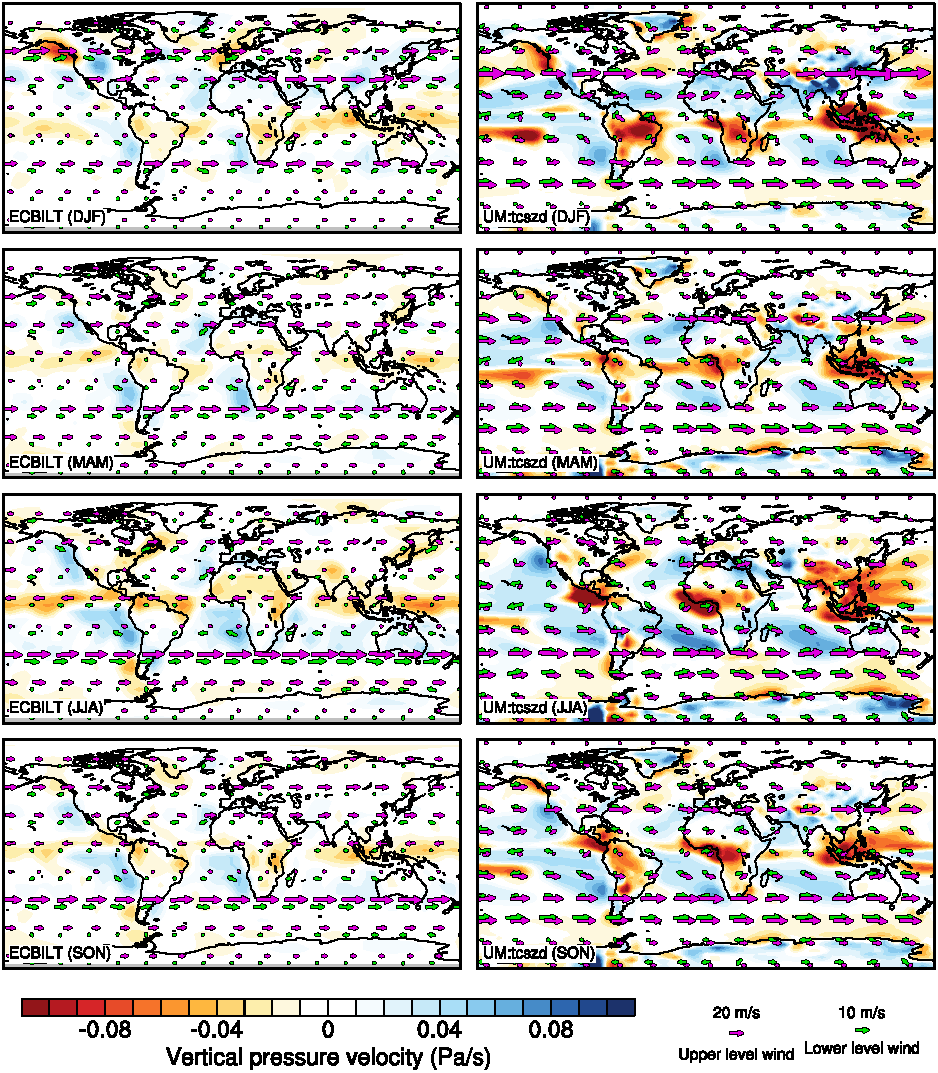
\includegraphics[width=\textwidth]{../control-expt-1/plots/wind-plots}
  \end{center}
  \caption{Seasonal circulation plots for ECBILT and UM comparison
    experiments: arrows show upper level and lower level winds,
    colours show middle atmosphere vertical pressure velocity.}
  \label{fig:wind}
\end{figure}

\end{document}
